\documentclass[ruledheader,noindentfirst,anapcustomindent,abntfigtabnum,tocpage=plain]{abnt}
\usepackage{amsmath, amssymb, amsthm, verbatim, amsfonts, amstext}
%\usepackage[latin1]{inputenc}
\usepackage[brazilian]{babel}
\usepackage[utf8]{inputenc}
\usepackage[T1]{fontenc}
\usepackage{dropping}
\usepackage{graphicx}
\usepackage[hang,small,bf]{caption}
\usepackage[abnt-etal-list=0,abnt-etal-text=it,abnt-and-type=&,abnt-emphasize=bf,abnt-full-initials=yes,alf,bibjustif]{abntcite}
\usepackage{fancyhdr}
\usepackage{makeidx}
\usepackage[none]{hyphenat}
\usepackage{color}
\usepackage{subfig}
\usepackage{algorithms}
\usepackage{algorithmic}
\usepackage{mdwlist}
\usepackage{bm}
\usepackage[titletoc,title]{appendix}
\usepackage{ltxtable}
\usepackage{longtable}
\usepackage{supertabular}
\usepackage{indentfirst}
\usepackage{color}
\usepackage{icomma}

\sloppy


%
%Tradução do pacote Algorithm para portugues
%
\renewcommand{\algorithmicrequire}{\textbf{Entrada:}}
\renewcommand{\algorithmicensure}{\textbf{Saída:}}
\renewcommand{\algorithmicend}{\textbf{fim}}
\renewcommand{\algorithmicif}{\textbf{se}}
\renewcommand{\algorithmicthen}{\textbf{então}}
\renewcommand{\algorithmicelse}{\textbf{senão}}
\renewcommand{\algorithmicelsif}{\algorithmicelse \, \algorithmicif}
\renewcommand{\algorithmicendif}{\algorithmicend \, \algorithmicif}
\renewcommand{\algorithmicfor}{\textbf{para}}
\renewcommand{\algorithmicforall}{\textbf{para todo}}
\renewcommand{\algorithmicdo}{\textbf{fazer}}
\renewcommand{\algorithmicendfor}{\algorithmicend \, \algorithmicfor}
\renewcommand{\algorithmicwhile}{\textbf{enquanto}}
\renewcommand{\algorithmicendwhile}{\algorithmicend \, \algorithmicwhile}
\renewcommand{\algorithmicloop}{\textbf{laço}}
\renewcommand{\algorithmicendloop}{\algorithmicend \, \algorithmicloop}
\renewcommand{\algorithmicrepeat}{\textbf{repetir}}
\renewcommand{\algorithmicuntil}{\textbf{até}}
\renewcommand{\algorithmiccomment}[1]{\{#1\}}
\renewcommand{\listalgorithmname}{Lista de Algoritmos}
\floatname{algorithm}{Algoritmo}
%%%%%%%%%%%%%%%%%%%%%%%%%%%%%%%%%%%%%%%%%%%%%%%%%%%%%%%%%%%%%%%%%%%%%%%%%%%%%%%%%%%

\makeindex

%%%% O arquivo modelosCAP.tex possui as definições para ciação do estilo de capítulo (fonte de título, barras horizontais, etc.)
% ele não gera texto de saída, é um arquivo de configuração somente
%
%Estilo de formatação de capítulos

\makeatletter
\newcommand{\thechapterwords}
{ \ifcase \thechapter\or 1\or 2\or 3\or 4\or 5\or6\or 7\or 8\or 9\or 10\or 11\fi}

\def\@makechapterhead#1{%
\vspace*{10\p@}%
{\parindent \z@  \reset@font

\scshape \@chapapp{} \thechapterwords
\quad %
\par\nobreak
\vspace*{10\p@}%
\interlinepenalty\@M
\hrule
\vspace*{10\p@}%
\Huge \bfseries #1\par\nobreak
\par
\vspace*{10\p@}%
\hrule
\vskip 40\p@
}}
\def\@makeschapterhead#1{%
\vspace*{10\p@}%
{\parindent \z@ \centering \reset@font
\par\nobreak
\vspace*{10\p@}%
\interlinepenalty\@M
\hrule
\vspace*{10\p@}%
\Huge \bfseries #1\par\nobreak
\par
\vspace*{10\p@}%
\hrule
\vskip 40\p@
%\vskip 100\p@
}}
%%%%%%%%%%%%%%%%%%%%%%%%%%%%%%%%%%%%%%%%%%%%%%%FIM DO PREAMBULO%%%%%%%%%%%%%%%%%%%%%%%%%%%%%%%%%%%%%%%%%%%%%%%%%%%%%%%%%%%%%%%%%%


\begin{document}

%%%%% IMPORTANTE: ALTERA O TEXTO ENTRE ARIAL E TIMES NEW ROMAN (ALTERNAR OS COMENTÁRIOS)
%
%%%%%%%%%%%%%%%%%%%%%PARA UTILIZAR ARIAL%%%%%%%%%%%%%%%%%%%%%%%
%
\fontfamily{phv}                    %fonte Arial
\renewcommand{\rmdefault}{phv}      %
%
%%%%%%%%%%%%%%%%%%%%%PARA UTILIZAR TIMES%%%%%%%%%%%%%%%%%%%%%%%
%
%\fontfamily{ptm}               %fonte Times
%\renewcommand{\rmdefault}{ptm} %
%
%%%%%%%%%%%%%%%%%%%%%%%%%%%%%%%%%%%%%%%%%%%%%%%%%%%%%%%%%%%%%%%

%%%%%%%%%%%%%Arquivos .tex com os elementos pré-textuais
%
\thispagestyle{empty}

\vfill
 \begin{center}
    \begin{figure}[t]
     \centering
            
\includegraphics[width=5cm]{figures/IF_logo.eps}\\[-0.1in]
     \end{figure}

    {\large\bfseries INSTITUTO FEDERAL DE EDUCAÇÃO, CIÊNCIA E TECNOLOGIA DO CEARA} \\
    {\large\bfseries PRÓ-REITORIA DE ENSINO} \\
    {\large\bfseries COORDENADORIA DE TELEMÁTICA DO CAMPUS MARACANAÚ}  \\ 
    {\large\bfseries BACHARELADO EM CIÊNCIA DA COMPUTAÇÃO}  \\ 

    \vspace*{1in}
    \begin{large} \bfseries FELIPE MARCEL DE QUEIROZ SANTOS \end{large}\\[0.4in]

    \vspace*{4cm}
    \noindent \\
    \large\bfseries{TÍTULO DO TRABALHO} \\
    \vfill
    \large\bfseries{ MARACANAÚ \\ 2015}
\end{center}

\normalsize
\begin{titlepage}
\vfill
\begin{center}

    {\large FELIPE MARCEL DE QUEIROZ SANTOS\\}
    \vspace{2cm}
    {\Large \textsc{TiTULO DO TRABALHO}\\}
    \vspace{1cm}
    \hspace{.45\linewidth}
    \begin{minipage}{.50\linewidth}

            Monografia submetida à Coordenadoria de Telemática e à Coordenadoria do Curso de Bacharelado 
            em Ciência da Computação do Instituto Federal do Ceará - Campus Maracanaú, como requisito 
            parcial para obtenção do grau de Bacharel em Ciência da Computação.

            \vspace{0.5 cm}

            Área de pesquisa: Aprendizagem de Máquina

            \vspace{0.5 cm}

            Orientador:D.r AMAURI HOLANDA SOUZA JUNIOR
    
    \end{minipage}

    \vspace{2cm}
    \vfill
    {\large Maracanaú\\ 2015}
\end{center}

\end{titlepage}
\begin{folhadeaprovacao}
\setlength{\ABNTsignthickness}{0.2pt}
\setlength{\ABNTsignskip}{1.7cm}

\begin{center}

\includegraphics[width=2.5cm]{figures/brasao_republica.eps}\\
            {ESCOLA POLITÉCNICA DA USP} \\

    \vspace{1.5cm}
                                    {NOME DO ALUNO}\\
    \bfseries{}
\end{center}

Esta Monografia foi julgada adequada para a obtenção do Grau de Bacharel em Ciência da Computação, sendo aprovada pela Coordenadoria de Telemática e pela Coordenadoria do curso de Bacharelado em Ciência da Computação do Campus Maracanaú do Instituto Federal de Educação, Ciência e Tecnologia do Ceará e pela banca examinadora:

    \vspace{0.15cm}
    \assinatura{Orientador: Prof. Dr. Amauri \\ Instituto Federal do Ceará - IFCE}
    \assinatura{Prof. Dr. Huguinho \\ Instituto Federal do Ceará - IFCE}
    \assinatura{Prof. Dr. Zezinho \\ Instituto Federal do Ceará - IFCE}
    \assinatura{Prof. Dr. Luizinho \\ Instituto Federal do Ceará - IFCE}
    \vspace{0.15cm}%\vfill

    \begin{center}
        Fortaleza, 06 de Abril de 2013
    \end{center}
\end{folhadeaprovacao}
\vspace*{15cm}

\hfill Dedico este trabalho ...\\
\chapter*{Agradecimentos}
%\thispagestyle{empty}


\begin{flushright}
\begin{minipage}[r]{10cm}
\vspace{18cm}
``A mente que se abre a uma nova idéia jamais voltará ao seu tamanho original''.
\begin{flushright}
Albert Einstein
\end{flushright}
\end{minipage}
\end{flushright}
\pagestyle{plain}%%%%% Utilizar ESTILO PLAIN AQUI%%%%%%%
\chapter*{Resumo}

\noindent Este trabalho apresenta...
\chapter*{Abstract}


\noindent This work presents...

%%%Comandos para criação automática das listas
%
\tableofcontents
\listoffigures
\listoftables

%%%Comandos para criar outras listas não suportadas pelo pacote ABNTex%%%
%
\pretextualchapter{Lista de Símbolos}
\begin{basedescript}{\desclabelstyle{\pushlabel}\desclabelwidth{6em}}
\item[$Z$] variavel aleatoria%
\item[$\mathbb{R}$] conjunto dos números reais%
\item[$t$] tempo contínuo%
\item[$n$] tempo discreto%
\item[$f(z)$] função densidade de probabilidade%
\item[$F(z)$] função de distribuição acumulada%
\item[$\sigma$] desvio padrão%
\item[$\mu$] média ou esperança matemática%
\item[$|\cdot|$] operador magnitude%
\item[$\nabla$] operador gradiente%
\end{basedescript}
\newpage

\pretextualchapter{Lista de Abreviacoes}
\begin{basedescript}{\desclabelstyle{\pushlabel}\desclabelwidth{6em}}
\item[{fdp}] Função densidade de probabilidade%
\item[{fda}] Função de distribuição acumulada%
\item[{EMQ}] Erro médio quadrático%
\end{basedescript}
\newpage
%%%%%%%%%%%%%%%%%%%%%%%%%%%%%%%%%%%%%%%%%%%%%%%%%%%%%%%%%%%%%%%%%%%%

%Capítulos passam a ter páginas numeradas
%
\pagestyle{fancy}

%resseta os contadores de capítulo e seção
%
\renewcommand{\chaptermark}[1]{\markboth{#1}{}}
\renewcommand{\sectionmark}[1]{\markright{\thesection\ #1}}

%%%%%%%%%%%%%%NÃO LEMBRO O QUE FAZ, APARENTEMENTE NADA, TESTAR DEPOIS
%\fancyhf{}%
%\fancyhead[RO,LE]{\large\slshape\thepage}%
%\fancyhead[CE]{\large\slshape\leftmark}%
%\fancyhead[CO]{\large\slshape\rightmark}%


%%% Outros arquivos .tex. É acoselhável utilizar vários arquivos, pelo menos um por capítulo
\chapter{Introdução}\label{CAP:introducao}
%\thispagestyle{empty}

% Este documento consiste de um modelo basico para a producao de documentos academicos, seguindo as normas ABNT. 

% Nao e abordado o estudo do LaTex neste template. Sugerimos a leitura do texto em \citeonline{Oetiker:1995}. O uso do LaTex e aconselhavel devido a sua qualidade grafica, facil referenciacao, criacao de listas, indices, referencias bibliograficas e escrita matematica profissional. Porem, nao e obrigatorio o uso deste template, apenas as orientacoes de formatação segundo as normas ABNT devem ser obrigatoriamente seguidas.

% Uma observação em particular é a de que, no pacote ABNTex, as referências diretas devem utilizar o comando ``citeonline''. Referências indiretas utilizam o comando ``cite''.

% Exemplo de citacao direta: Uma otima fonte de estudo para compreender o LaTex e apresentada por \citeonline{Oetiker:1995}. 

% Exemplo de citação indireta: Existem boas fontes de pesquisa para entendimento do LaTex \cite{Oetiker:1995}, estas incluem documentação online disponível na web.
blablabla

\section{Objetivos}


 
\section{Diferenças UML e SysML}




\sectioan{Uso}


\section{História}

Com o intuito de elaborar uma linguagem unificada de propósito geral para engenharia de sistemas, diante das limitações da UML (Unified Modeling Language) a SysML foi criada pelo Object Management Group (OMG) em conjunto com o International Council on Systems Engineering (INCOSE). 

Em 2003, foram publicados os requisitos de uma linguagem de modelagem que servisse para Engenharia de Sistemas, criando-se, em seguida, um grupo de trabalho composto por representantes da indústria e produtores de ferramentas CASE chamado SysML Partners. Esse grupo ficou responsável por desenvolver a linguagem respeitando os requisitos estabelecidos. 

Em 2004 foi publicada a versão draft da SysML e em 2005 a versão SysML 1.0. A versão formal pública SysML OMG v 1.2 foi publicada pela  OMG em Junho de 2010. Desde então a linguagem vem se tornando cada vez disseminada e aceita pela comunidade se mostrando adequada para as demandas de Engenharia de Sistemas.

Assim surgiu a SysML, como uma extensão da UML V2 que expande a proposta de programação orientada a objetos possibilitando a representação de requisitos do sistema, componentes que não são de softwares, equações, fluxos contínuos e alocações.


\noindent \textbf{Capitulo \ref{CAP2}}: descricao...

\noindent \textbf{Capitulo \ref{CAP3}}: descricaoo...

\noindent \textbf{Capitulo \ref{CAP4}}: descricao...

\noindent \textbf{Capitulo \ref{CAP5}}: descricao...
\chapter{Métodos de Kernel}
\label{CAP2}


Este capítulo tem como objetivo 


\section{Kernel em análise de padrões}\label{Sub:equa}

Em análise de padrões, temos como objetivo detectar automaticamente padrões em um conjunto de dados de um determinado problema. Por padrões, podemos entender qualquer relação ou regularidades inerentes à alguma estrutura em uma fonte de dados. Essa análise geralmente é feita a partir dos valores de entrada e suas respectivas saídas(no caso da aprendizagem supervisionada) fornecidas no problema. Essas informações podem formar padrões em que se torna possível verificar o valor de uma saída dada uma nova entrada fornecida pelo usuário. 

Diversos problemas podem ser resolvidos utilizando esta abordagem, categorização de textos, análise de sequências de DNA, reconhecimento de escrita, por exemplo.

A abordagem de análise de padrões utilizando métodos de kernel se baseia em adaptar os dados de entrada em um espaço característico adequado e nos algoritmos usados para descobrir os padrões do problema. Levando em conta isso, podemos pensar que qualquer solução com métodos de kernel é composta por estas duas partes: uma em que é feito o mapeamento nesse espaço característico e a outra em que é executado o algoritmo de aprendizagem para detectar os padrões neste espaço. A ideia por trás desta abordagem é poder mapear os dados em um espaço em que possamos 

Uma das principais caracerísticas desses métodos é o atalho computacional que pode ser utilizado, tal atalho é conhecido como função de kernel.


O Kernel  é uma função de mapeamento de dados em dimensões superiores com a motivação de torná-los mais fáceis de separar ou estruturá-los de maneira mais adequada. Essas funções podem ser utilizadas nas tarefas de reconhecimento de padrões. 

\begin{equation}\label{Eq:multiplicacao}
%
Z = X \cdot Y,
%
\end{equation}
%
em que $Z$, $X$ e $Y$ são variáveis complexas. A referenciação à Equação (\ref{Eq:multiplicacao}) é feita por meio do comando ``ref''. O mesmo vale para outros tipos de elementos.

\subsection{Exemplo de uma equação mais complexa}

  Equações mais complexas podem ser mais facilmente escritas com uso do programa TexAide. Como, por exemplo,

    \begin{equation}\label{Eq:sqrt_gamma_X}
    f_{\Gamma ^{{1 \mathord{\left/
    {\vphantom {1 2}} \right.
    \kern-\nulldelimiterspace} 2}} } (x;\alpha ,\lambda ) = \frac{{2\lambda ^\alpha  }}{{\Gamma (\alpha )}}x^{2\alpha  - 1} \exp \left( { - \lambda x^2 } \right).
    \end{equation}
    \[
    \alpha ,\lambda > 0.
    \]
    %
    em que $\Gamma(\cdot)$ é a função Gama. O programa TexAide é semelhante ao \textit{MathType} do Office, porém ao copiar e colar a equação em um arquivo tex, é gerado o código em LaTex referente a esta equação.

\section{Tabelas}

Tabelas são essenciais na apresentação de dados. A Tabela \ref{Tb:X_models} mostra um exemplo do uso deste tipo de elemento. Vale ressaltar que não é aconselhável o uso de linhas verticais em trabalhos acadêmicos e de pesquisa.

\begin{table}[h]
 \caption{Modelos estatísticos e suas relações.}%
 \label{Tb:X_models}
  \centering
\begin{tabular}{c c c c c}
 \hline
 &&&&\\
                                             &$\alpha ,\lambda  > 0$    &                               &$\alpha ,\lambda \rightarrow\infty$  &Homogêneo \\
                                             &$\gamma  \to 0$           & Heterogêneo                   &$\alpha / \lambda \rightarrow \beta$ & \\
                                             &$\mathop  \to \limits^D $ & $\sqrt\Gamma(\alpha,\lambda)$ &$\mathop  \to \limits^P $            &$\sqrt\beta$        \\
$\mathcal{N}^{-1/2}(x;\alpha,\gamma,\lambda)$& & & &\\
                                             &$\mathop  \to \limits^D $ & $\Gamma^{-1/2}(\alpha,\gamma)$&$\mathop  \to \limits^P $   &$\sqrt{\zeta^{-1}}$ \\
                                             &$\lambda \to 0$           &  Extremamente                 &$-\alpha / \gamma \rightarrow \zeta^{-1}$ & \\
                                             &$-\alpha ,\gamma   > 0$   &  Heterogêneo                  &$-\alpha ,\gamma \rightarrow\infty$ &Homogêneo \\
 &&&& \\
 \hline
 &&&&\\
                                             &$\alpha ,\lambda  > 0$    &                               &$\alpha ,\lambda \rightarrow\infty$  &Homogêneo \\
                                             &$\gamma  \to 0$           & Heterogêneo                   &$\alpha / \lambda \rightarrow \beta$ & \\
                                             &$\mathop  \to \limits^D $ &$\mathcal{K}_A(\alpha,\lambda,n)$&$\mathop  \to \limits^P $&$\sqrt\Gamma(n,n/\beta)$        \\
$\mathcal{G}_A(z;\alpha,\gamma,\lambda,n)$   & & & &\\
                                             &$\mathop  \to \limits^D $ & $\mathcal{G}_A^0(\alpha,\gamma,n)$&$\mathop  \to \limits^P $&$\sqrt\Gamma(n,n\zeta)$  \\
                                             &$\lambda \to 0$           &  Extremamente                 &$-\alpha / \gamma \rightarrow \zeta$ & \\
                                             &$-\alpha ,\gamma   > 0$   &  Heterogêneo                  &$-\alpha ,\gamma \rightarrow\infty$ &Homogêneo \\
&&&&   \\
 \hline

\end{tabular}
\end{table}


A Figura \ref{Fig:1} mostra o exemplo do uso do comando ``subfigure''. Apesar de aceitar diferentes tipos de imagens. É preferível que as imagens estejam no formato .eps. Isso garante que a imagem impressa seja exatamente aquela visualizada, como acontece com arquivos pdf.

\begin{figure}[!ht]
\centering
\subfloat[]{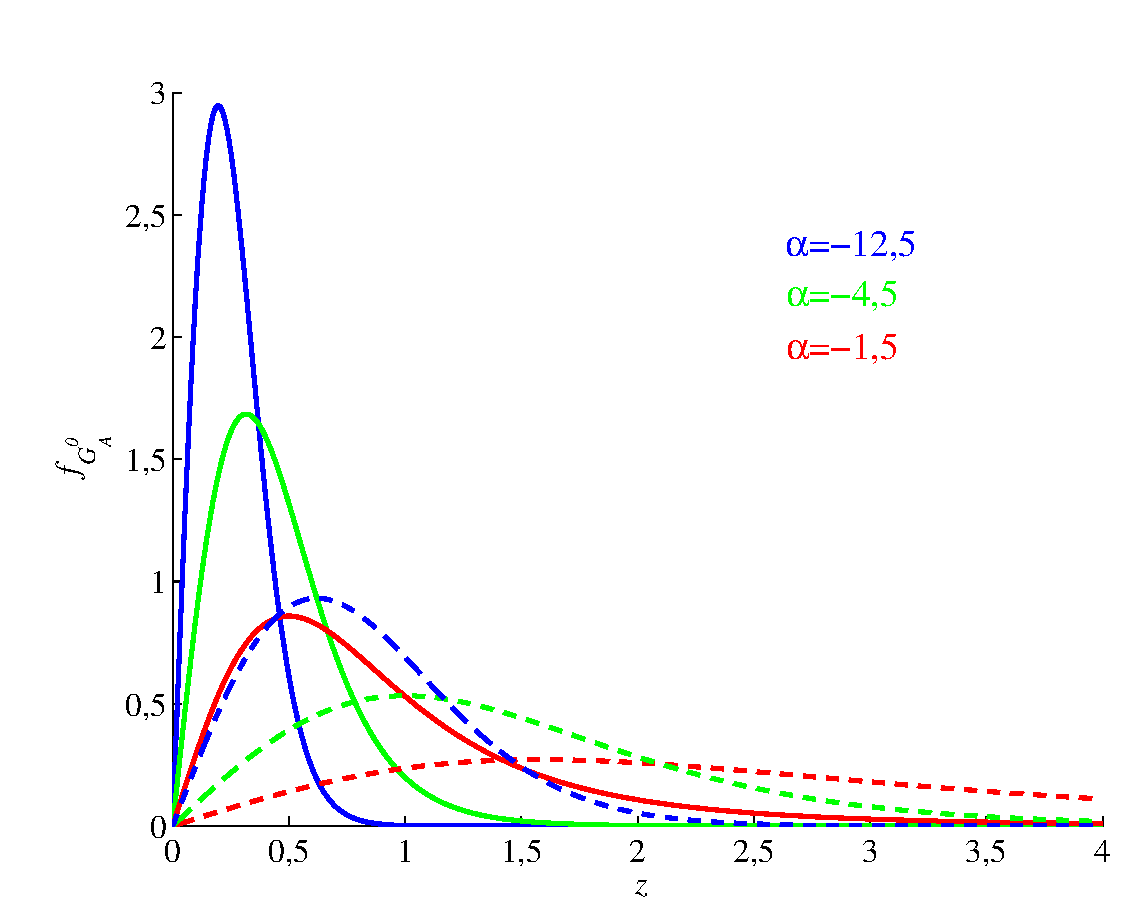
\includegraphics[scale=.65]{figures/fig1.eps}}\\
\subfloat[]{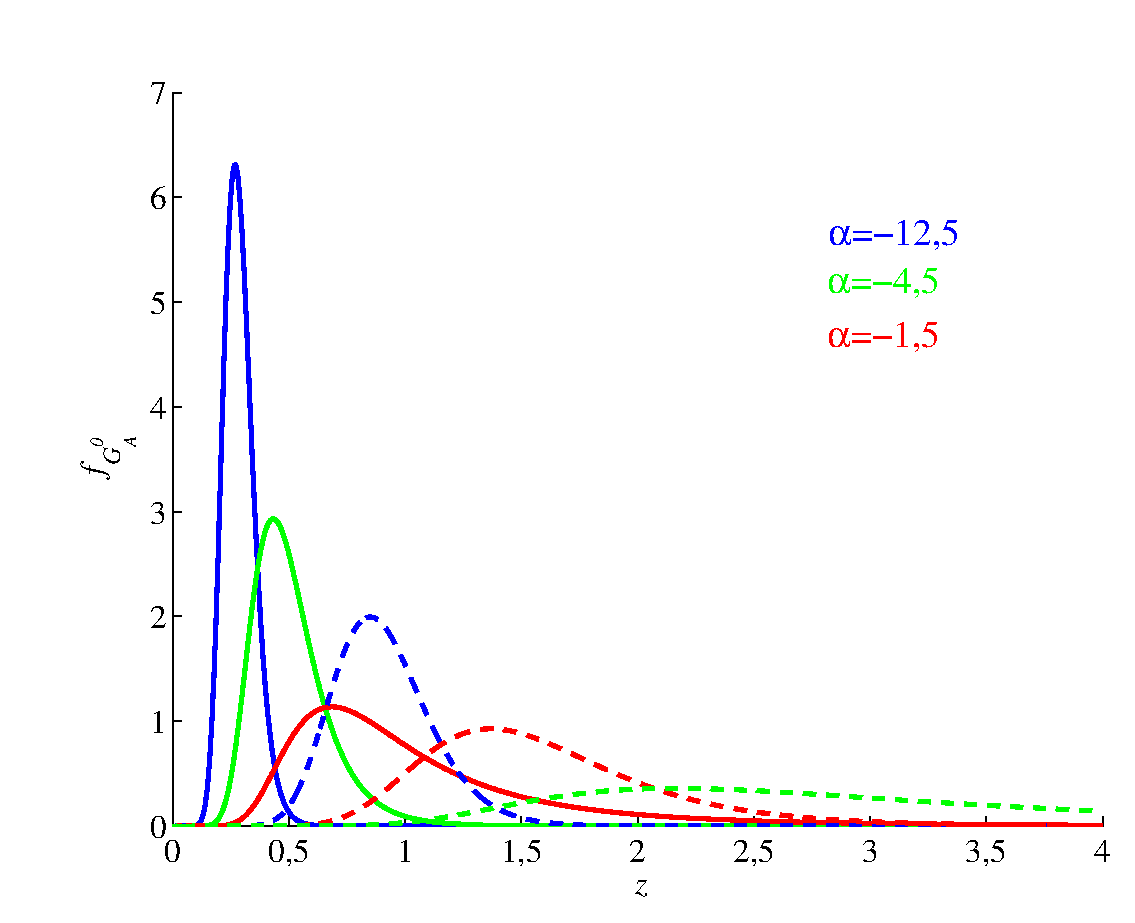
\includegraphics[scale=.65]{figures/fig2.eps}}
\caption{ Curvas de funções de probabilidade: (a) exemplo 1, (b) exemplo 2.} \label{Fig:1}
\end{figure}
\chapter{Método Proposto}\label{CAP3}
\chapter{Resultados Experimentais}\label{CAP4}
\chapter{Conclusão e Trabalhos Futuros}\label{CAP5}


%%%% Estilo de citação ABNT e arquivo de bibitens (mybibliography.bib)
\bibliographystyle{abnt-alf}
\bibliography{mybibliography}

\apendice
\chapter{Título do Apêndice}
\label{Apx:A}




\chapter{Exemplo do pacote Algorithm}
\label{Apx:B}


\begin{algorithm}[!h]
\caption{Estimador ML otimizado.}\label{Alg:MAXVER}
\begin{algorithmic}[1]
\STATE Inicializar o contador: $j\leftarrow 1$;%
\STATE Fixar o limiar de variação das estimativas: $e_{\mathrm{out}}\leftarrow 10^{-4}$;%
\STATE Fixar o número máximo de iterações: $N\leftarrow 1000$;%
\STATE Computar o ponto inicial: $\hat \gamma(0)$;%
\STATE Determinar o limiar inicial: $e_1 \leftarrow1000$;%
\STATE Estabelecer o valor inicial de $\alpha$: $\hat \alpha(0) \leftarrow -10^{-6}$;%
\WHILE{ $e_j \geq e_{\mathrm{out}}$ e $ j\leq M$}
    \STATE Solucionar $\hat \alpha_j\leftarrow {\arg \max}_{\alpha}\;{l_1(\alpha; \gamma_{j-1},\mathbf{z},n)}$;%
    \STATE Solucionar $\hat \gamma_j\leftarrow {\arg \max}_{\gamma}\;{l_2(\gamma; \alpha_j,\mathbf{z},n)}$;%
    \STATE $j\leftarrow j+1$
    \STATE Computar o critério de convergência: $e_j$;%
\ENDWHILE
\end{algorithmic}
\end{algorithm}


\end{document}